
%% bare_jrnl.tex
%% V1.4b
%% 2015/08/26
%% by Michael Shell
%% see http://www.michaelshell.org/
%% for current contact information.
%%
%% This is a skeleton file demonstrating the use of IEEEtran.cls
%% (requires IEEEtran.cls version 1.8b or later) with an IEEE
%% journal paper.
%%
%% Support sites:
%% http://www.michaelshell.org/tex/ieeetran/
%% http://www.ctan.org/pkg/ieeetran
%% and
%% http://www.ieee.org/

%%*************************************************************************
%% Legal Notice:
%% This code is offered as-is without any warranty either expressed or
%% implied; without even the implied warranty of MERCHANTABILITY or
%% FITNESS FOR A PARTICULAR PURPOSE! 
%% User assumes all risk.
%% In no event shall the IEEE or any contributor to this code be liable for
%% any damages or losses, including, but not limited to, incidental,
%% consequential, or any other damages, resulting from the use or misuse
%% of any information contained here.
%%
%% All comments are the opinions of their respective authors and are not
%% necessarily endorsed by the IEEE.
%%
%% This work is distributed under the LaTeX Project Public License (LPPL)
%% ( http://www.latex-project.org/ ) version 1.3, and may be freely used,
%% distributed and modified. A copy of the LPPL, version 1.3, is included
%% in the base LaTeX documentation of all distributions of LaTeX released
%% 2003/12/01 or later.
%% Retain all contribution notices and credits.
%% ** Modified files should be clearly indicated as such, including  **
%% ** renaming them and changing author support contact information. **
%%*************************************************************************


% *** Authors should verify (and, if needed, correct) their LaTeX system  ***
% *** with the testflow diagnostic prior to trusting their LaTeX platform ***
% *** with production work. The IEEE's font choices and paper sizes can   ***
% *** trigger bugs that do not appear when using other class files.       ***                          ***
% The testflow support page is at:
% http://www.michaelshell.org/tex/testflow/

% formatting instructions
% https://ras.papercept.net/conferences/support/files/IEEEtran_HOWTO.pdf

% from here
%https://journals.ieeeauthorcenter.ieee.org/create-your-ieee-journal-article/authoring-tools-and-templates/ieee-article-templates/templates-for-transactions/
%\UseRawInputEncoding
\documentclass[journal]{IEEEtran}

\usepackage{cite}
\usepackage{amsmath}
\usepackage{url}
\usepackage{multirow}
% don't use the borders around links
\usepackage[hidelinks]{hyperref}
\usepackage{listings}

% *** GRAPHICS RELATED PACKAGES ***
%
\ifCLASSINFOpdf
  \usepackage[pdftex]{graphicx}
  % declare the path(s) where your graphic files are
\graphicspath{{../images/}}
  % and their extensions so you won't have to specify these with
  % every instance of \includegraphics
  % \DeclareGraphicsExtensions{.pdf,.jpeg,.png}
\else
  % or other class option (dvipsone, dvipdf, if not using dvips). graphicx
  % will default to the driver specified in the system graphics.cfg if no
  % driver is specified.
  % \usepackage[dvips]{graphicx}
  % declare the path(s) where your graphic files are
  % \graphicspath{{../eps/}}
  % and their extensions so you won't have to specify these with
  % every instance of \includegraphics
  % \DeclareGraphicsExtensions{.eps}
\fi

\begin{document}

\title{A Datalake Solution for\\ 
       Time Series Data}

\author{Paul~Adams, paula@smu.edu,
        Rikel~Djoko, rdjoko@smu.edu,
        and Stuart Miller, stuart@smu.edu}

% The paper headers
\markboth{MSDS7330 Term Paper}
{MSDS7330 Term Paper}
% The only time the second header will appear is for the odd numbered pages
% after the title page when using the twoside option.

% make the title area
\maketitle

% This should be about 150-200 words
\begin{abstract}

In this paper, we present a solution for warehousing structured and semi-structured 
financial markets time series data.
Traditional systems, such as SQL databases, are well suited for storing highly structured data,
 but were not designed to store semi-structured forms of data.
Additionally, traditional systems, which operate with ACID transactions,
 can be slow over large volumes of data.
"Big Data" systems were developed to store this type of data,
 addressing this gap in data storage system technology.
We developed a system to store structured and semi-structured time series data based on the 
 Apache Hadoop ecosystem.
Based on the results of testing read query performance,
 schema denormalization and increasing the Hadoop cluster size will reduce query times.
A distributed data warehouse framework like Hadoop could be used in cases where data scaling is expected,
 requiring the computing infrastructure to scale with the data.

\end{abstract}

\section{Introduction}

% - paragraph 1 – motivation; set the stage
% - This is the topic and this is why it is important
% - don’t be too specific

\IEEEPARstart{T}{h}e ability to capture and generate large volumes of data is an issue
 many enterprises face.
The increase in data generation and recording is often referred to as "Big Data."
Traditionally, data generation systems were slow and the data was easily structured, 
 which lent to the use of traditional systems.
However, "Big Data" is often semi-structured or unstructured and
 can be generated at high rates,
  such as server logs or real-time sensor data \cite{Intel}.
"Big Data" technologies were developed to address the gap between the current type of data
 that are generated and collected and capacity of traditional storage tools \cite{BigDataComputing}.
These "Big Data" technologies are able to collect data in raw form and
provide access to the data, often using languages similar to Structured Query Languages (SQL).

% - paragraph 2 – the specific problem

An example of "Big Data" is financial market data and
 related "alternative" data that may be useful for prediction.
For alternative data to be useful to a prediction system,
 it must be stored in a system that can provide low query time.
Additionally, it must be able to work with data that does not follow strict structuring,
 such as text-based messages or images.
In financial market modeling, alternative data is any type of data outside the
 financial domain \cite{xiao2018trading}.
An application of financial market prediction using alternative data is
 utilizing Twitter data to make predictions on the stock market \cite{twittermood}.
A data storage system would need to store large volumes of time series data and
 provide rapid query access to those volumes to support a financial 
 market prediction engine.
In this paper, we will present a "Big Data" system that can be used to store and
 access large volumes of time series data. 
Stock data, intraday and daily,
 will be the primary time series used in the analysis.
Data from Twitter will serve as the primary source of alternative data.
For this analysis, we collected approximately four-hundred thousand tweets from over 
one-hundred Twitter accounts and approximately 49 million stock data points.

% - paragraph 3 and beyond - your solution

The Hadoop ecosystem is at the core of this system.
Hadoop is an open source framework for distributed computing
 that is sponsored by the 
 Apache Software Foundation\footnote{https://hadoop.apache.org/} \cite{HDFSarchitecture}.
Since Hadoop is a distributed computing framework,
 the server cluster used in the implementation can be horizontally scaled to
 accommodate the need for more computing power as the data storage grows.
The Hadoop ecosystem consists of modules for file storage, data warehousing,
 data flow, data analysis, and machine learning.
The primary components of Hadoop used in this system are
 Hadoop Distributed File System (HDFS) and Hive.

HDFS is a file system distributed over multiple servers (a server cluster) \cite{HDFSarchitecture}.
The processing framework that enables this is called MapReduce, 
 which assigns nodes for ``mapping'' and ``reducing'' processes by applying  
 various configurations, such as related to memory allocation and numbers
 of mappers and reducers \cite{MappingReducing}.
As data is mapped, it is reprocessed into a derivative data set,
 split into tuples that are then processed across the cluster, in parallel,
 and reassembled in the reduce process \cite{MappingReducing}.
Hive is a distributed data warehouse that manages data stored in HDFS \cite{HDFSarchitecture}.
Hive provides an SQL-like query language to access and
 retrieve the data stored in HDFS.

We implemented the solution with Amazon Web Services (AWS),
 which provides a set of cloud services for data storage and warehousing.
Elastic MapReduce (EMR) is a preconfigured service for Hadoop provided by AWS.
EMR runs on a cluster of Elastic Compute 2 (EC2) servers,
 which can be horizontally scaled as needed.
We used EMR for the physical implementation of the Hadoop ecosystem in this project.

We designed two schemas for the data warehouse in a star configuration.
The first schema was designed in a fully normalized fashion,
 which is known as a snowflake schema.
Our second schema was based on the snowflake schema, 
 but denormalized to limit the number of tables, 
 which limits the number of joins required in queries.
Query performance will be measured on these schemas to determine
 which how much improvement is provided by schema denormalziation.

We will test the performance of this system implementation with the collected stock and 
 Twitter data. 
Performance of the data warehouse is based on time taken to process the data queried in the Hive 
 warehouse.
The analysis will examine the improvement in performance from the schema denormalization and
 increasing the EMR cluster size.
We will use a two-way analysis of variance (ANVOA) to compare the differences
 in combinations of schema and EMR cluster size.

\section{Data}

We collected stock data and Twitter data for this study.
Both daily and intraday stock price data were collected
 for use in this analysis. 
Twitter\footnote{https://www.twitter.com/}
 was chosen as the primary source of alternative data because of
 ease-of-access to the 
 \href{https://developer.twitter.com/en/docs}{Twitter API}\footnote{https://developer.twitter.com/en/docs}
 and the large volume of available data.
Categories of data are summarized in Table \ref{DataCategories} and a full
 list of features is given in Appendix \ref{DataFeatures}.


\subsection{Stock Data}

The stock price data was collected through an API provided by
 \href{https://www.alphavantage.co/}{Alpha Vantage}\footnote{https://www.alphavantage.co/}.
The R\footnote{Version 3.6.1}
 programming language was used to collect data from the Alpha Vantage API,
 using the R package alphavantager\footnote{https://cran.r-project.org/web/packages/alphavantager/index.html}
\cite{R}.
This API provided access to daily prices, intraday stock prices,
 and intraday price features from the following categories Bollinger bands, 
 stochastic oscillators, moving averages, and exponential moving averages. 

The stock data was collected from Oct. 04, 2019 to Oct. 24, 2019 on
 all 2520 symbols traded on the NYSE and all 3213 symbols traded on the NASDAQ.
A single value was stored for each feature of the daily prices.
The intraday values were sampled at 15 minute intervals from market open
 to market close.
This resulted in a total of 49,093,917 stock data points.

\subsection{Twitter Data}

Messages on Twitter (called tweets) are mainly comprised of
 tweet ID, timestamp, user (screen name), and text.
Tweets can also contain many other features such as
 URLs, hashtags, emojis,  and mentions.
For this analysis, in addition to the main features,
 URLs, hashtags, and mentions were also collected in the data warehouse.
A mention is a reference to another Twitter user's screen name
 in the text of a tweet.
A hashtag is some collection of characters starting with
 '\#' without white space.
Generally, the character portion of a hashtag will be a word or set of words,
 but this is not necessary.
An example of a tweet containing one hashtag (\texttt{\#FF}) and one 
mention (\texttt{@everett}) is given in Listing \ref{SampleTweet} (the value of
 '\texttt{full\_text}').

\begin{table}
	\renewcommand{\arraystretch}{1.3}
	\caption{Data Categories}
	\label{DataCategories}
	\centering
	\begin{tabular}{c l}
		\hline
		\hline
		\textbf{Source}       & \textbf{Features}\\
		\hline
		\multirow{3}{*}{Stock Daily} &  Symbol \\
		&  Time Stamp \\
		&  Prices \\
		\hline
		\multirow{6}{*}{Stock Intraday} &  Symbol \\
		&  Time Stamp \\
		&  Prices \\
		&  Bollinger Bands \\
		&  Moving Averages \\
		&  Stochastic Indicators \\
		\hline
		\multirow{7}{*}{Twitter} &  Symbol \\
		&  Time Stamp \\
		&  User \\
		&  Text \\
		&  URLs \\
		&  Hashtags \\
		&  Mentions \\
		\hline
		\hline
	\end{tabular}
\end{table}

We collected 423,802 tweets from 108 Twitter users, using the
 python\footnote{Version 3.6.8}
 module Twython\footnote{https://pypi.org/project/twython/3.6.0/}.
The data from Twitter is returned in JavaScript Object Notation (JSON); 
 an example is shown in Listing \ref{SampleTweet}.
The features of interest were extracted from the JSON files and reformatted in tab
 separated files (TSV) using python and the built-in JSON and CSV modules.
After the tweets were extracted from Twitter,
 mentions of company names or stock symbols were extracted from the tweet text by
 matching sections of tweet text to company names and company stock symbols.
All other featured were extracted from the JSON by key.

\lstset{
	breaklines=true,
	emph={
		created\_at,
	    full\_text,
	    id\_str,
	    entities,
	    hashtags,
	    urls,
	    user\_mentions,
	    user,
	    expanded\_url,
	    text,
	    screen\_name
      },
	emphstyle=\textbf
}

% example tweet json; this is a fake
\begin{lstlisting}[frame=single,
 caption={Sample Tweet JSON},
 label={SampleTweet}]
{'created_at': 'Fri Oct 25 07:44:38 +0000 2019',
 'id': 1187636067505188864,
 'id_str': '1187636067505188864',
 'full_text': '@everett where do I start with this company? #FF!!!!',
 'truncated': False,
 'display_text_range': [0, 52],
 'entities': {
   'hashtags': [
            {'text': 'FF',
             'indices': [45, 48]}],
   'symbols': [],
   'user_mentions': [
          {'screen_name': 'even_everett',
           'name': 'Even Everett',
           'id': 21841004,
           'id_str': '21841004',
           'indices': [0, 10]}],
   'urls': [
     "indices": [32, 52],
     "url": "http://t.co/TZR",
     "display_url": "you.com/watch?v=oHg…",
     "expanded_url": "http://www.you.com/watch?v=TZR"]}
 'user': {'id': 14216123,
   'id_str': '14216123',
   'name': 'Jim Jim',
   'screen_name': 'jimjim',
   ...}
}
\end{lstlisting}

As shown in Listing \ref{SampleTweet}, the timestamp, text, and tweet ID
 can be accessed at the top level of the JSON object with \texttt{created\_at},
 \texttt{full\_text}, and \texttt{id\_str}, respectively. 
The user information can be accessed from the key \texttt{user}, 
 which accesses another set of objects. 
The values for \texttt{screen\_name} and \texttt{id\_str} were extracted for the user.
The hashtags, mentions, and URLs are located under the key \texttt{entities} as
 \texttt{hashtags}, \texttt{user\_mentions}, and \texttt{urls}, respectively.
Each of these keys under \texttt{entities}, return an array of objects,
 containing the features of interest. 
The value for \texttt{text} under \texttt{hashtags} was the only value collected
 for the hashtags (\texttt{\#FF} in the example).
The values for \texttt{screen\_name} and \texttt{id\_str} under 
 \texttt{user\_mentions} were collected for mentions (\texttt{even\_everett} and
 \texttt{21841004}, respectively, in the example).
Only the value of \texttt{expanded\_url} was collected user \texttt{urls}
 (\texttt{http://www.you.com/watch?v=TZR} in the example).

\begin{figure}
	\centering
	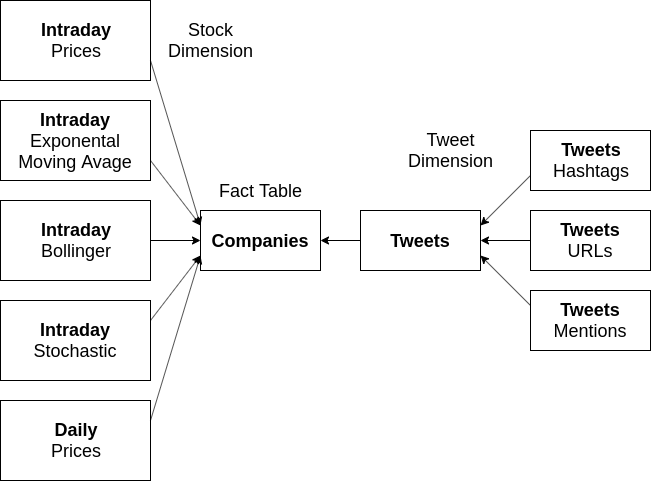
\includegraphics[width=2.5in]{SnowFlake_Schema_Simple.png}
	\caption{Conceptual Diagram of the Data Warehouse Snowflake Schema}
	\label{snowflake}
\end{figure}

\section{Data Warehouse Development}
\label{DataWarehouseDevelopment}

Data warehouses are often designed with a \textit{star} schema 
 \cite{BuildingtheDWCH11}.
In a star schema design, there is a central table (called the fact table),
 which contains the unifying features of the dataset and keys to other tables
 \cite{BuildingtheDWCH11}.
The tables surrounding the fact table (called dimension tables) 
 contain information related to a category of the facts \cite{Enterprise}.
In the dataset for this analysis, the unifying features are timestamp and
 company stock symbol.
The combination of timestamp and symbol is a natural key into the stock data and
 the twitter data.
These features were included on the fact table as the primary key.
The company name and exchange market associated with the symbols were 
 included on the fact table for convenience.
The natural dimensions of the fact table are intraday stock data,
 daily stock data, and tweet data.

In some cases, dimensions can be normalized into multiple tables. 
When the dimensions of a star schema are are normalized, the schema
 is in its \textit{snowflake} form \cite{WarehouseDesignApproaches}.
In this study, two schemas were designed: one in snowflake form and
 the other in a denormalized form.
We will consider a star schema in snowflake form when it is normalized into
 third normal form (3NF), meaning the domains of the attributes are atomic and
 there are no functional dependencies on a portion of the primary key \cite{DSCNormalization}.


\begin{figure}
	\centering
	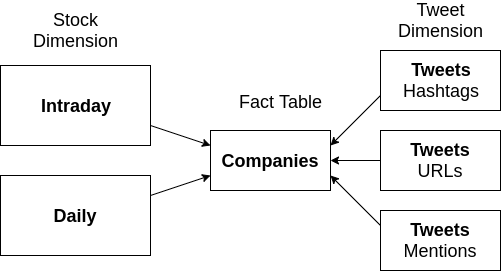
\includegraphics[width=2.5in]{Star_Schema_Simple.png}
	\caption{Conceptual Diagram of the Data Warehouse 
		Denormalized Star Schema}
	\label{star}
\end{figure}

\subsection{Snowflake Schema}

As noted previously, the fact table of this star design contained the
 company symbols and timestamps as a composite primary key.
The three dimensions of fact table, daily stock data, intraday stock data, and 
 tweet data, share the primary key of the fact table.

The stock data comes in a form suitable for the snowflake design; 
 it is already in 3NF.
However, the intraday data was split into five tables for a more 
 general use schema design: prices, Bollinger bands, moving averages,
 and stochastic indicators.
The daily stock table and the intraday stock tables are shown joining to the 
 fact table in Fig. \ref{snowflake} (left side of the schema diagram).

Like the stock data, the tweet data came with a timestamp, but stock symbol
 is not a nominal feature of tweets.
The stock symbol feature was generated by extracting matching strings
 during the data collection process; therefore, stock symbols are not
 guaranteed to be non-null in the tweet dimension.
Thus, the same features can still be used to join the tweet dimension to the 
fact table, but cannot serve as a primary key.
However, Twitter assigns a tweet ID for each tweet, which is guaranteed to be
 a primary key.
The tweet ID was used as the primary key of the tweet table.

As noted previously, three secondary features of tweets are used in this study.
Each of these features, mentions, hashtags, and URLs, is a normalizable
 feature of the tweet dimension.
To achieve a 3NF design, the unique attributes of the tweets were collected
 in a central table and tables were created for mentions, hashtags, and URLs.
Since there is a many-to-many cardinality between the central tweet table and each of 
 the three secondary members, join tables were created to connect the secondary tables 
 to the central tweet table. 
The result of the tweet dimension normalization is shown conceptually
 in Fig. \ref{snowflake} (right side of schema diagram).

\subsection{Denormalized Star Schema}

While the snowflake schema is suitable for general use cases.
The number of tables should be limited to decrease query read time to support
 fast data transfer to a machine learning system.
The number of intraday tables and tweet tables were reduced to support
 fast query times.
All intraday tables were combined into one table. 
Each secondary member of the normalized tweet dimension was
 subsumed into a copy of the main tweet table, reducing the number of tables
 in the tweet dimension from seven to three.
The schema resulting from this denormalization process is shown
 conceptually in Fig. \ref{star}.

\begin{figure}
	\centering
	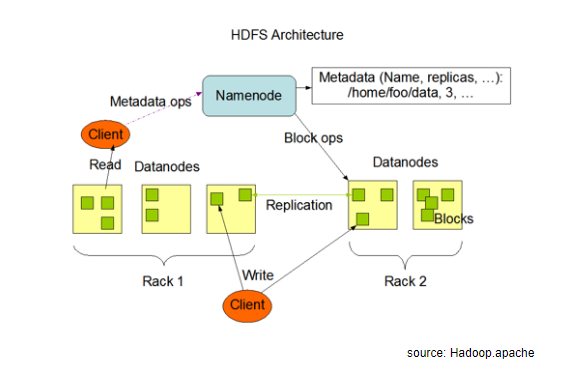
\includegraphics[width=3.5in]{HDFS_Arch.png}
	\caption{HDFS Architecture \cite{HDFS}}
	\label{HDFS}
\end{figure}

\section{Implementation}

Multiple vendors provide platforms and infrastructure for data warehousing technologies, 
 this project was implemented using Amazon Web Services (AWS).
AWS is a set of cloud computing services provided by Amazon.com\footnote{https://aws.amazon.com/}
 that are accessible over the internet.
AWS provides multiple services for many different applications. 
Elastic MapReduce (EMR) was used for the implementation of Hadoop in this project.

\subsection{AWS Elastic MapReduce}

AWS EMR is a pre-configured compute cluster for Big Data.
The cluster can be provisioned and terminated on demand as needed.
It comes with a configurable set of the Hadoop ecosystem elements pre-installed and ready to use.
The EMR cluster used in this study was provisioned with three
 m5.xlarge\footnote{https://aws.amazon.com/ec2/instance-types/m5/}
 elastic compute instances using version 5.27.0 of the EMR 
 software\footnote{emr-5.27.0 contains Amazon Hadoop 2.8.5, Hive 2.3.5, and Hue 4.4.0. See https://docs.aws.amazon.com/emr/latest/ReleaseGuide/emr-release-5x.html}.

\subsection{Apache Hadoop}

Hadoop is an open source software framework for the distributed storage and
 distributed processing of a very large datasets. 
The core of Apache Hadoop consists of a storage part: Hadoop Distributed File System
 (HDFS) and a processing part MapReduce.

\begin{figure}
	\centering
	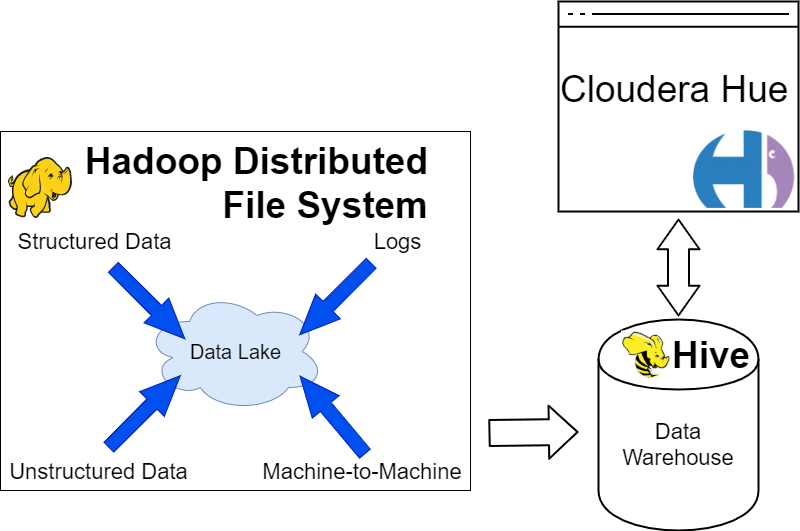
\includegraphics[width=2.7in]{system_overview_final.png}
	\caption{Overview of Data System}
	\label{system_overview_final}
\end{figure}

\subsubsection{Hadoop Distributed File System (HDFS) and  MapReduce}

Unlike traditional file systems, the Hadoop Distributed File System (HDFS) is a distributed file system designed to run on commodity hardware. 
HDFS architecture consists of a master node, called a "NameNode" and at least one slave node, called "DataNodes."\cite{HDFSarchitecture}.
The NameNode is the controller which consist storing data and metadata of the data no the DataNodes. 
The metadata includes a Namespace lookup table used to locate each file from the DataNodes, which assists in node cluster-computing. 

HDFS works by storing duplicate copies of data blocks across multiple servers. Those blocks are then split into chunks, which are then 
replicated across the cluster, partitioned by server rack. Data jobs take advantage of this feature by breaking down into tasks, 
where each task pairs with blocks of data and are therefore replicated across the cluster as well. If one job fails, it can be restarted 
by the other running tasks until all tasks have been completed and data compiled for the end-user \cite{HadoopAdmin}.

In reference to Fig. 3, the client - in our case, Hive, but this can be a different application supported by the Hadoop ecosystem - requests a 
read operation by passing blocks of HDFS files from Datanodes in Rack 1 with their associated metadata to the Namenode, which then delegates
block processing operations to the Datanodes in Rack 2. Tasks are assigned from the Namenode and partitioned across the racks. 
Although all data is in both racks - because write operations replicate data across the racks, as indicated in Fig. 3 - each rack has unique tasks
to operate. In the event a task fails in a node, another node will resume the task since the data is duplicated \cite{HadoopAdmin}. 

\subsubsection{Hadoop MapReduce}

Hadoop MapReduce is a programming model for large scale data processing. With MapReduce, instead of using one server instance with multiple 
processors, multiple servers with multiple processors are used for computation. This is refers to a distributed computing system.

MapReduce uses the divide and conquer technique where the input is divided into a set of small tasks. Each task is identified by a key-value 
pair \cite{Divide-and-Conquer}. The key serves as a task ID and the value as the task output. Each task is then processed and executed by the 
mapper and the outputs are processed and merged by the reducer \cite{MapReduce}. MapReduce couples with HDFS to enable horizontal
scaling in a cluster-computing environment.

\subsection{AWS Simple Storage Service}

As the name implies, the S3 is a storage system.
It is used to store and retrieve any amount of data any time, from anywhere on the web. 
S3 is reliable, fast, and inexpensive.

\subsection{Apache Hive}

Apache Hive is a data warehouse application built on top of Hadoop. We used Hive to structure, organize, model, and query our data using the Hive 
Query Language, HQL. We structured files from within the Hadoop Distributed File System (HDFS) and loaded them into tables within Hive. 
Hive operates by using the HDFS storage to generate tables. However, when Hive queries are executed, the data is retrieved from HDFS via the compiler, 
which uses an execution engine and metastore to return results. \cite{Hivemetastore}

\subsection{Cloudera Hue}

Cloudera Hue\footnote{https://gethue.com/}
 is an open source web application that served as user interface for Hadoop components.
Hue provides access to Hadoop from within a browser, allowing users to interact with the Hadoop ecosystem applications. 
Hue is an alternative to accessing the Hadoop ecosystem applications from the command line interface.
Hue was used to interact with the EMR cluster and run Hive scripts.

\subsection{System Design}
Once fully configured, the system we developed included three- or five-node EMR clusters.
Data collected by members of our team were stored in Amazon S3.
The data was loaded into HDFS from S3 prior to creating structured tables in Hive.
Local hosts would connect to the Namenode master server by SSH to allow interfacing with Hue.
Hive tasks would be executed on the EMR cluster from the Hue interfaces to create and load the data warehouse (as shown in Fig. 4).

\section{Study Design}
\label{StudyDesign}

In this study, we will investigate the impact of schema normalization and
 EMR cluster size on the performance of a read query.
Both schemas presented in Section \ref{DataWarehouseDevelopment} were tested on
 EMR clusters with 3 nodes and 5 nodes.
This is a two-way ANOVA where ERM cluster size and schema
 are the explanatory factor variables and the response variable is query
 execution time \cite{RepeatMeasures}.

During performance testing, we gathered all fields from all tables,
 joining all tables in the schema together. 
Joining all tables enabled capturing the entirety of the database,
 under each schema, to produce the same results. 
These queries were limited to 75,000 returned records to enable gathering more runtime samples. 
This number was decided to be reasonable based on the difference in performance time. 
As noted in the analysis section below,
 the performance time between queries was significant at 75,000 records;
 limited a higher volume of returned records would have increased the significance. 
Therefore, 75,000 was determined reasonable for analysis.


\begin{table}
	\renewcommand{\arraystretch}{1.3}
	\caption{Results Table}
	\label{ResultsTable}
	\centering
	\begin{tabular}{c c c c}
		\hline
		\hline
		\multirow{2}{*}{\textbf{Schema}} & \multirow{2}{*}{\textbf{Cluster Nodes}} &
		\multicolumn{2}{c}{\textbf{Query Time} (seconds)}   \\
		\cline{3-4}
		&     & Mean & Standard Deviation\\
		\hline
		\multirow{2}{*}{Snowflake}         & 3   & 121.05 & 4.12 \\
		
		& 5   & 94.49 & 4.01  \\
		
		\hline
		\multirow{2}{*}{Denormalized Star} & 3   & 103.77 & 2.99 \\
		
		& 5   & 79.68 & 5.86  \\
		
		\hline
		\hline
	\end{tabular}
\end{table}

\section{Results}

As discussed in Section \ref{StudyDesign}, a two-way ANOVA test was performed.
We identified that the interaction between schema design and server count provide significant results,
indicating that there is a difference in the proportions of performance speed between the two schemas when considering count of servers in a cluster.
The dependence of performance on combinations of schema and cluster size is apparent in Fig. \ref{Results},
 which shows boxplots of the query times of each combination of schema and cluster size.
The red boxes represent the query times for the snowflake schema and
 the blue boxes represent the query times for the denormalized schema.
The boxplot is faceted by cluster size with the three-node results on the right and
 the five-node results on the left.
The query time of the denormalized schema is lower than the normalized schema for both sizes of clusters.

We find that, while holding cluster size constant,
 schema design is significant on performance across both server sizes
 (p-value $< 0.0001$, F $ = 999.187$). 
Denormalizing the snowflake schema provided a 14.27\% decrease in mean query time on
 the three-node cluster and a 15.67\% decrease mean in query time on the five-node cluster.
Furthermore, while holding schema design constant, 
 performance speed difference was also significant 
 (p-value $< 0.0001$, F $= 3399.954$) 
 between the two cluster sizes with the five-node cluster outperforming
 the three-node cluster. 
A summary of the results is shown in Table \ref{ResultsTable}.

\begin{figure}
	\centering
	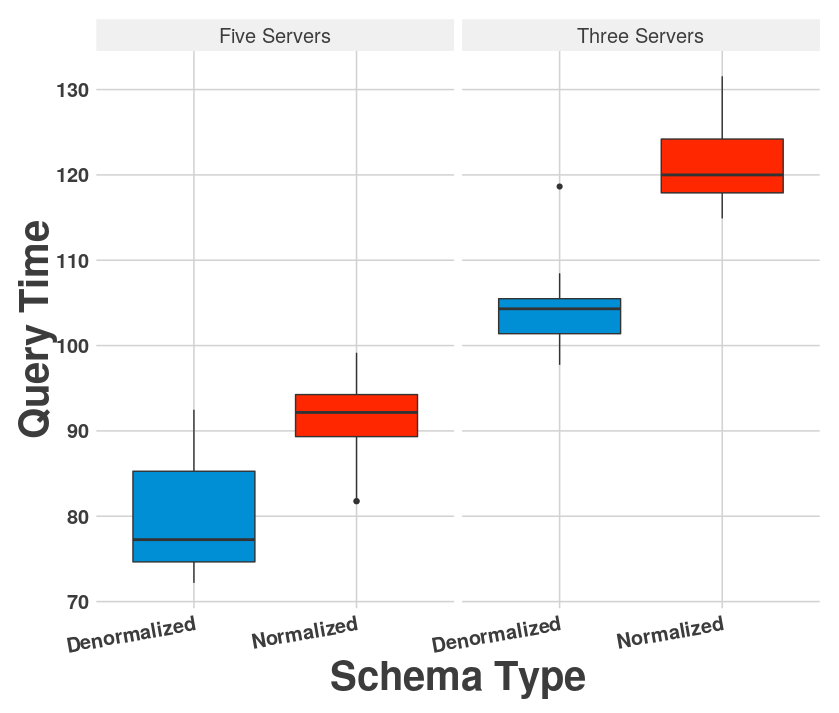
\includegraphics[width=3.3in]{Rplot.png}
	\caption{Average of Query Time by Schema and Block Size with Standard Deviation Bars}
	\label{Results}
\end{figure}

\section{Analysis}

In analyzing the exploratory graphical analysis of the clusters, 
 the interaction between schema and cluster size is such that as cluster size increases,
 the normalized schema approaches a similar level of performance. 
However, testing indicates there is still a statistically significant difference between 
 performance at the five-server cluster level. 
Further testing could identify that, while holding database size constant, at some server level, 
 the normalized schema may outperform the de-normalized schema. 
However, this is based on linear approximation that may become non-linear with more samples and clusters. 
Regardless, under both cluster sizes,
 the de-normalized schema outperformed the normalized schema by a level of statistical significance.

\section{Conclusions}

With the increase in data collection activities,
 data storage systems will need to provide results of read queries on large datasets.
This analysis shows that query times of distributed data warehouses can be reduced by denormalizing the schema or 
 scaling up the number of servers in the physical implementation.
While schema denormalization does provide improvements for read queries,
 migration to a new schema may not be possible
 or may introduce other undesirable effects because the data definition and manipulation logic will be affected.
Since the logical design of the warehouse is abstracted from the physical implementation,
 increasing cluster size would be a better solution.
If read performance improvement on a distributed data warehousing system is needed,
 we recommend increasing the cluster size of the physical system. 

% Can use something like this to put references on a page
% by themselves when using endfloat and the captionsoff option.
\ifCLASSOPTIONcaptionsoff
  \newpage
\fi

\appendices

\section{Data Features}
\label{DataFeatures}

This section contains a full listing of all the features collected for this
 study. The features are listed by general category as shown in 
 Table \ref{DataCategories}.

\subsection{Daily Stock Features}

The daily stock features are described below and are organized in the
 following categories: Key Values and Prices.
The value for time was imputed to a standard value for the daily values.

\subsubsection{Key Values}

\begin{itemize}
	\item Symbol
	\item Time
	\item Date
\end{itemize}

\subsubsection{Prices}

\begin{itemize}
	\item Open
	\item Close
	\item High
	\item Low
\end{itemize}

\subsection{Intraday Stock Features}

The intraday stock features are described below and are organized in the 
 following categories: Key Values, Prices, Bollenger Bands, Moving Averages, and
  Stochastic Indicators.

\subsubsection{Key Values}

\begin{itemize}
	\item Symbol
	\item Time
	\item Date
\end{itemize}

\subsubsection{Prices}

\begin{itemize}
	\item Open
	\item Close
	\item High
	\item Low
\end{itemize}

\subsubsection{Bollenger Bands}

\begin{itemize}
	\item Open Lower Band
	\item Open Middle Band
	\item Open Upper Band
	\item Close Lower Band
	\item Close Middle Band
	\item Close Upper Band
	\item High Lower Band
	\item High Middle Band
	\item High Upper Band
	\item Low Lower Band
	\item Low Middle Band
	\item Low Upper Band
\end{itemize}

\subsubsection{Moving Averages}

\begin{itemize}
	\item Open Convergence Divergence
	\item Open Convergence Divergence Signal
	\item Open Convergence Divergence Historical
	\item Open Exponential
	\item Close Convergence Divergence
	\item Close Convergence Divergence Signal
	\item Close Convergence Divergence Historical
	\item Close Exponential
	\item High Convergence Divergence 
	\item High Convergence Divergence Signal
	\item High Convergence Divergence Historical
	\item High Exponential
	\item Low Convergence Divergence
	\item Low Convergence Divergence Signal
	\item Low Convergence Divergence Historical
	\item Low Exponential
\end{itemize}

\subsubsection{Stochastic Indicators}

\begin{itemize}
	\item 5-day indicator
	\item 3-day indicator
\end{itemize}

\subsection{Twitter Features}

The twitter features are described below and are organized in the
following categories: Unique and Common.
Unique features are specific to a particular tweet and
 common features are shared across many tweets.

\subsubsection{Unique}

\begin{itemize}
	\item Tweet ID
	\item Timestamp
	\item User (Author)
	\item Text
\end{itemize}

\subsubsection{Common}

\begin{itemize}
	\item Hashtags
	\item URLs
	\item User Mentions
\end{itemize}

\begin{thebibliography}{1}

\bibitem{BigDataComputing}
R. Kune, P. Konugurthi, A. Agarwal, R. Chillarige, R. Buyya,
 "The Anatomy of Big Data Computing," Software: Practice and Experience,
 Vol. 46 no. 1, pp.79-105, Jan. 2016. 

\bibitem{BuildingtheDWCH11}
W. H. Inmon, "Unstructured Data and the Data Warehouse," in 
  \emph{Building the Data Warehouse},
  4th ed. Hoboken: Wiley, 2005, ch. 11.
  Accessed on Nov. 6, 2019 [Online]. 
  Available: \\ https://learning.oreilly.com/library/view/building-the-data/9780764599446

\bibitem{WarehouseDesignApproaches}
I. Moalla, A. Nabli, L. Bouzguendam and M. Hammami,
 "Data warehouse design approaches from social media: review and comparison,"
 Social Network Analysis and Mining., Vol. 7, no. 1, pp. 1-14, Jan. 2017.
 Accessed on: Nov. 6, 2019 [Online]. 
 Available doi: 10.1007/s13278-017-0423-8

\bibitem{Enterprise}
A. Gorelik, "Historical Perspectives," in 
 \emph{The Enterprise Big Data Lake},
 1st ed. Sebastopol, CA: Wiley, 2019, ch. 2, pp. 25-47.

\bibitem{Intel}
 "Extract, Transform, and Load Big Data with Apache Hadoop," Intel, USA, 2013.
 Available:\\ https://software.intel.com/sites/default/files/article/402274/etl-big-data-with-hadoop.pdf

\bibitem{HadoopAdmin}
S. Alapati, Expert Hadoop Administration, 1st ed. Boston, MA: Addison-Wesley, 2017.

\bibitem{HDFS}
D. Borthakur, HDFS Architecture Guide, The Apache Software Foundation,
 August 22 2019. Accessed on: Nov. 8, 2019. [Online] Available: \\
 https://hadoop.apache.org/docs/r1.2.1/hdfs\_design.html

\bibitem{Parallelism}
D. Sitaram, G. Manjunath \textit{Moving To The Cloud}. Boston: Syngress, 2012, pp. 205–253.

\bibitem{Divide-and-Conquer} 
S. Zhao, R. Li, W. Tian, W. Xiao, X. Dong, D. Liao, S. U. Khan, L. Keqin, 
 “Divide-and-conquer approach for solving singular value decomposition based on MapReduce,” Abbrev. Title of Journal, vol. 28, no. 2, pp. 331–350, Nov. 2016. 
 Accessed on: Nov. 10, 2019 [Online]. Available: doi:10.1002/cpe.3436.

\bibitem{MapReduce}
D. Miner, A. Shook, MapReduce Design Patterns, 1st ed. Sebastopol, CA: O'Reilly Media, 2012,
 pp. 5–6.

\bibitem{MappingReducing}
D. Miner, A. Shook, Hadoop MapReduce v2 Cookbook, 2nd ed. Sebastopol, CA: O'Reilly Media,
 2015, pp. 1.

\bibitem{Hivemetastore}
 H. Bansal, S. Chauhan, S. Mehrota, Apache Hive Cookbook, 1st ed. Birmingham, UK: Packt Publishing, Limited, 2016.

\bibitem{HDFSarchitecture}
T. White, Hadoop: The Definitive Guide, 1st ed. Sebastopol,
 CA: O'Reilly Media, 2009, pp. 44.

\bibitem{R}
R Core Team, R: A language and environment for Statistical Computing, Vienna, Austria: 2018.
 Available: https://www.R-project.org/
 
\bibitem{Sleuth}
F. Ramsey and D. Schafer, "Repeated Measures and Other Multivariate Responses," 
 in \textit{The Statistical Sleuth}, 3rd ed. Boston: Brooks/Cole, 2013,
 ch. 16, pp. 479-485.  

\bibitem{RepeatMeasures}
M. Crawley, "Analysis of Variance," in \textit{The R Book},
 1st ed. Chichester, West Sussex, United Kingdom: Wiley, 2013,
 ch. 11, pp. 470-478.

\bibitem{OptimizeHadoop}
K. Tannir, "Enhancing Map and Reduce Tasks," in 
 \textit{Optimizing Hadoop for MapReduce},
 1st ed. Birmingham, England: Packt Publishing Ltd, 2014,
 ch. 5. Accessed on: Nov. 20, 2019 [Online]. 
 
\bibitem{DSCNormalization}
A. Silberschatz, H. Korth, and S. Sudarshan, "Relational Database Design," in
 \textit{Database Design Concepts}, 6th ed. NY: McGraw-Hill, 2011, ch. 8, sec. 8.3,
 pp. 329 - 338. 

\bibitem{xiao2018trading}
C. Xiao and W. Chen, “Trading the Twitter Sentiment with Reinforcement Learning,”
 arXiv:1801.02243v1 [cs.AI], Jan. 2018. Accessed on: Dec. 7, 2019 [Online].
 Available: https://arxiv.org/pdf/1801.02243.pdf.

\bibitem{twittermood}
J. Bollen and H. Mao. "Twitter mood as a stock market predictor,"
 Computer, Vol. 44, no. 10, pp. 91–94, 2011. Accessed on: Dec. 7, 2019 [Online].
 Available: doi: 10.1109/MC.2011.323


\end{thebibliography}



% that's all folks
\end{document}


